\documentclass[aspectratio=169]{beamer}
% Including necessary packages for equations, figures, and formatting
\usepackage{graphicx}
\usepackage{amsmath, amssymb}
\usepackage{hyperref}
\usepackage{caption}
\usepackage{subcaption}
\usepackage{booktabs}
\usepackage{listings}
\usepackage{xcolor}
\usepackage{algorithm}
\usepackage{algpseudocode}
\usepackage{tikz}
\usepackage{multicol}
\usepackage{pgfplots}
\usepackage{minted}
\usepackage{amsfonts}
\usepackage{bm}

% Setting the theme and colors for a professional look
\usetheme{default}
\usecolortheme{default}
\setbeamertemplate{navigation symbols}{}
\setbeamertemplate{footline}[frame number]

% Setting up the title page information
\title{Majorana Zero Modes Modelling and Simulation}
\subtitle{MT-507 - Modelling and Simulation in Material Science (JAN-JUNE 2025)}
\author{Atharva Thombare (B23365) \and Shejul Nikhil Ravindra (B23386)}
\institute{Indian Institute of Technology, Mandi \\ School of Mechanical And Materials Engineering \\ Submitted to: Dr. Dube Dheeraj Prakashchand Sir}
\date{Submission Date: 10-5-25}
\titlegraphic{\includegraphics[width=3cm]{logo.png}}

% Beginning the document
\begin{document}

% Creating the title slide
\maketitle

% Introducing the 1D Kitaev Chain
\begin{frame}{1D Kitaev Chain Hamiltonian}
The 1D Kitaev chain is a model for topological superconductors, describing a spinless chain of $N$ lattice sites with nearest-neighbor hopping and $p$-wave pairing. The Hamiltonian captures the physics of Majorana Zero Modes (MZMs), which are zero-energy edge states with potential applications in topological quantum computing.
\[ H = -\mu \sum_{j=1}^N c_j^\dagger c_j - t \sum_{j=1}^{N-1} \bigl(c_j^\dagger c_{j+1} + c_{j+1}^\dagger c_j\bigr) + \Delta \sum_{j=1}^{N-1} \bigl(c_j c_{j+1} + c_{j+1}^\dagger c_j^\dagger\bigr). \]
\end{frame}

% Presenting the BdG formulation - Nambu spinor
\begin{frame}{Bogoliubov--de Gennes (BdG) Formulation}
To analyze the Kitaev chain, we use the BdG formalism, which accounts for particle-hole symmetry. We define the Nambu spinor to represent both particle and hole degrees of freedom:
\[ \Psi_j = \begin{pmatrix} c_j \\ c_j^\dagger \end{pmatrix}, \]
where $c_j$ and $c_j^\dagger$ are the annihilation and creation operators at site $j$.
\end{frame}

% Presenting the BdG Hamiltonian
\begin{frame}{BdG Hamiltonian}
The BdG Hamiltonian is a $2N \times 2N$ matrix that describes the system in the Nambu basis:
\[ H_{\mathrm{BdG}} = \begin{pmatrix} H_{\mathrm{kin}} - \mu I & \Delta_{\mathrm{p}} \\ \Delta_{\mathrm{p}}^\dagger & -\bigl(H_{\mathrm{kin}} - \mu I\bigr)^T \end{pmatrix}, \]
where $H_{\mathrm{kin}}$ includes hopping terms ($t$), $\mu$ is the chemical potential, and $\Delta_{\mathrm{p}}$ represents the $p$-wave pairing amplitude ($\Delta$).
\end{frame}

% Explaining diagonalization
\begin{frame}{Diagonalization for Quasiparticle States}
Diagonalizing the BdG Hamiltonian reveals the quasiparticle spectrum:
\[ H_{\mathrm{BdG}} \psi_n = E_n \psi_n. \]
We extract:
\begin{itemize}
\item $E_n$: Quasiparticle energies, where $E_n \approx 0$ indicates potential MZMs.
\item $\psi_n(j)$: Wavefunction amplitudes, showing spatial distribution of states.
\end{itemize}
MZMs are identified by zero-energy states localized at the chain's edges.
\end{frame}

% Defining localization length
\begin{frame}{Localization Length of Edge Modes}
For edge modes, the wavefunction amplitude $\psi(j)$ decays exponentially from the edge:
\[ |\psi(j)| \sim e^{-j / \xi}, \]
where $\xi$ is the localization length. Fitting this decay provides $\xi$, quantifying how tightly the MZM is confined to the edge, a key signature of topological protection.
\end{frame}

% Introducing the topological invariant
\begin{frame}{Topological Invariant: Winding Number}
The topological phase is characterized by the winding number $\nu$ under periodic boundary conditions:
\[ \nu = \frac{1}{2\pi} \int_{-\pi}^{\pi} \frac{\mathrm{d}\phi(k)}{\mathrm{d}k} \,\mathrm{d}k, \]
where $\phi(k) = \mathrm{Arg}\bigl[\det \Delta_{\mathrm{p}}(k)\bigr]$. A non-zero $\nu$ indicates a topological phase hosting MZMs.
\end{frame}

% Detailing the parameter sweep
\begin{frame}{Parameter Sweep for Dataset Generation}
To study MZM behavior, we sweep system parameters over uniform grids using \texttt{linspace}:
\[ \mu \in [\mu_{\min}, \mu_{\max}], \quad t \in [t_{\min}, t_{\max}], \quad \Delta \in [\Delta_{\min}, \Delta_{\max}], \]
\[ B \in [B_{\min}, B_{\max}], \quad \alpha \in [\alpha_{\min}, \alpha_{\max}]. \]
The dataset includes:
\[ \bigl(\mu, t, \Delta, B, \alpha; E_n, \psi_n, \xi, \nu\bigr), \]
enabling analysis of MZM occurrence across parameter space.
\end{frame}

% Listing variable definitions in two columns
\begin{frame}{Variable Definitions}
\begin{columns}
\begin{column}{0.5\textwidth}
\begin{description}
\item[$c_j^\dagger, c_j$] Creation/annihilation operators at site $j$.
\item[$\mu$] Chemical potential, controlling particle density.
\item[$t$] Hopping amplitude between nearest neighbors.
\item[$\Delta$] $p$-wave pairing amplitude, enabling superconductivity.
\item[$N$] Number of lattice sites in the chain.
\end{description}
\end{column}
\begin{column}{0.5\textwidth}
\begin{description}
\item[$E_n, \psi_n$] Eigenvalues/eigenvectors of $H_{\mathrm{BdG}}$, describing quasiparticles.
\item[$\xi$] Localization length, measuring edge mode confinement.
\item[$\nu$] Winding number, indicating topological phase.
\item[$B$] Zeeman field strength, introducing magnetic effects.
\item[$\alpha$] Spin-orbit coupling strength, affecting electron spin.
\end{description}
\end{column}
\end{columns}
\end{frame}

\begin{frame}{Edge-Localization Histogram}
  \tiny

  \begin{figure}
    \centering
    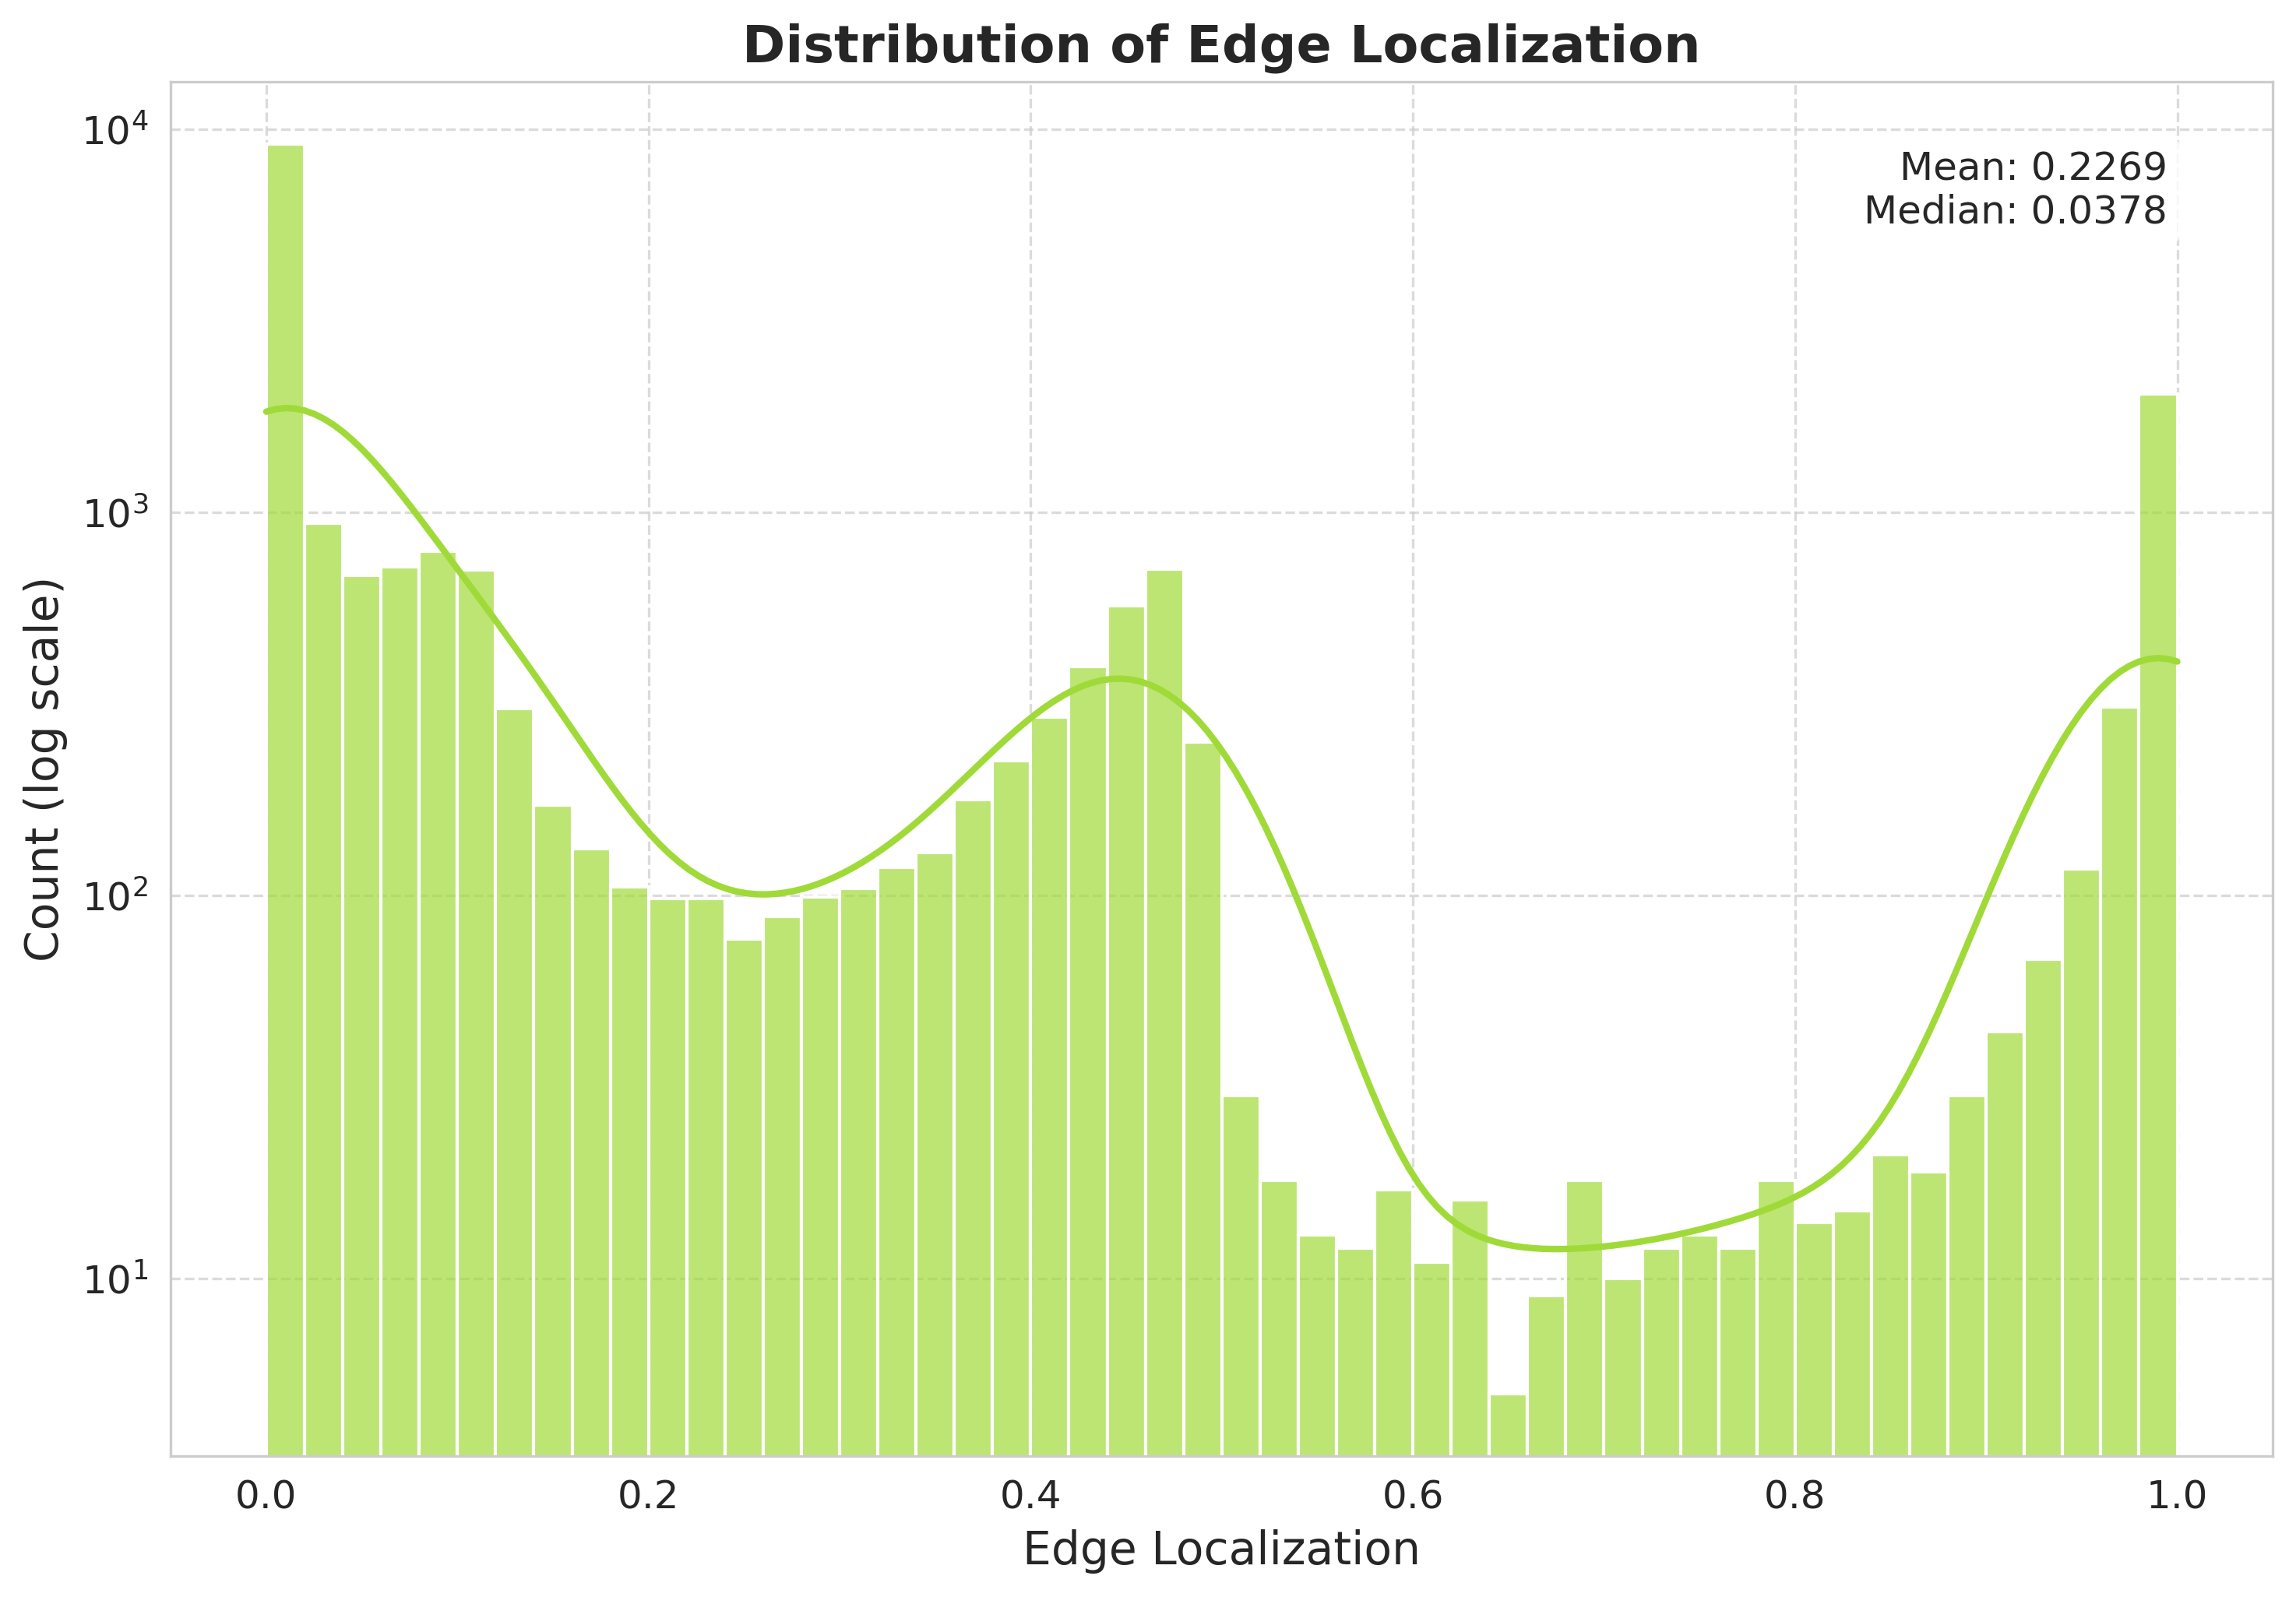
\includegraphics[width=0.65\textwidth]{edge_loc_hist.png}
    \captionsetup{labelformat=empty,font=tiny}
    \caption{Edge-localization histogram. The $x$-axis is the normalized localization metric (0 = bulk; 1 = edge), and the $y$-axis shows the sample count (log scale).}
  \end{figure}
  This histogram reveals an almost trimodal-like distribution, indicating states are either bulk-like or edge-localized, with MZMs appearing at the edge (metric $\approx 1$).
\end{frame}

\begin{frame}{PCA of Raw Binned Spectra}
  \tiny

  \begin{figure}
    \centering
    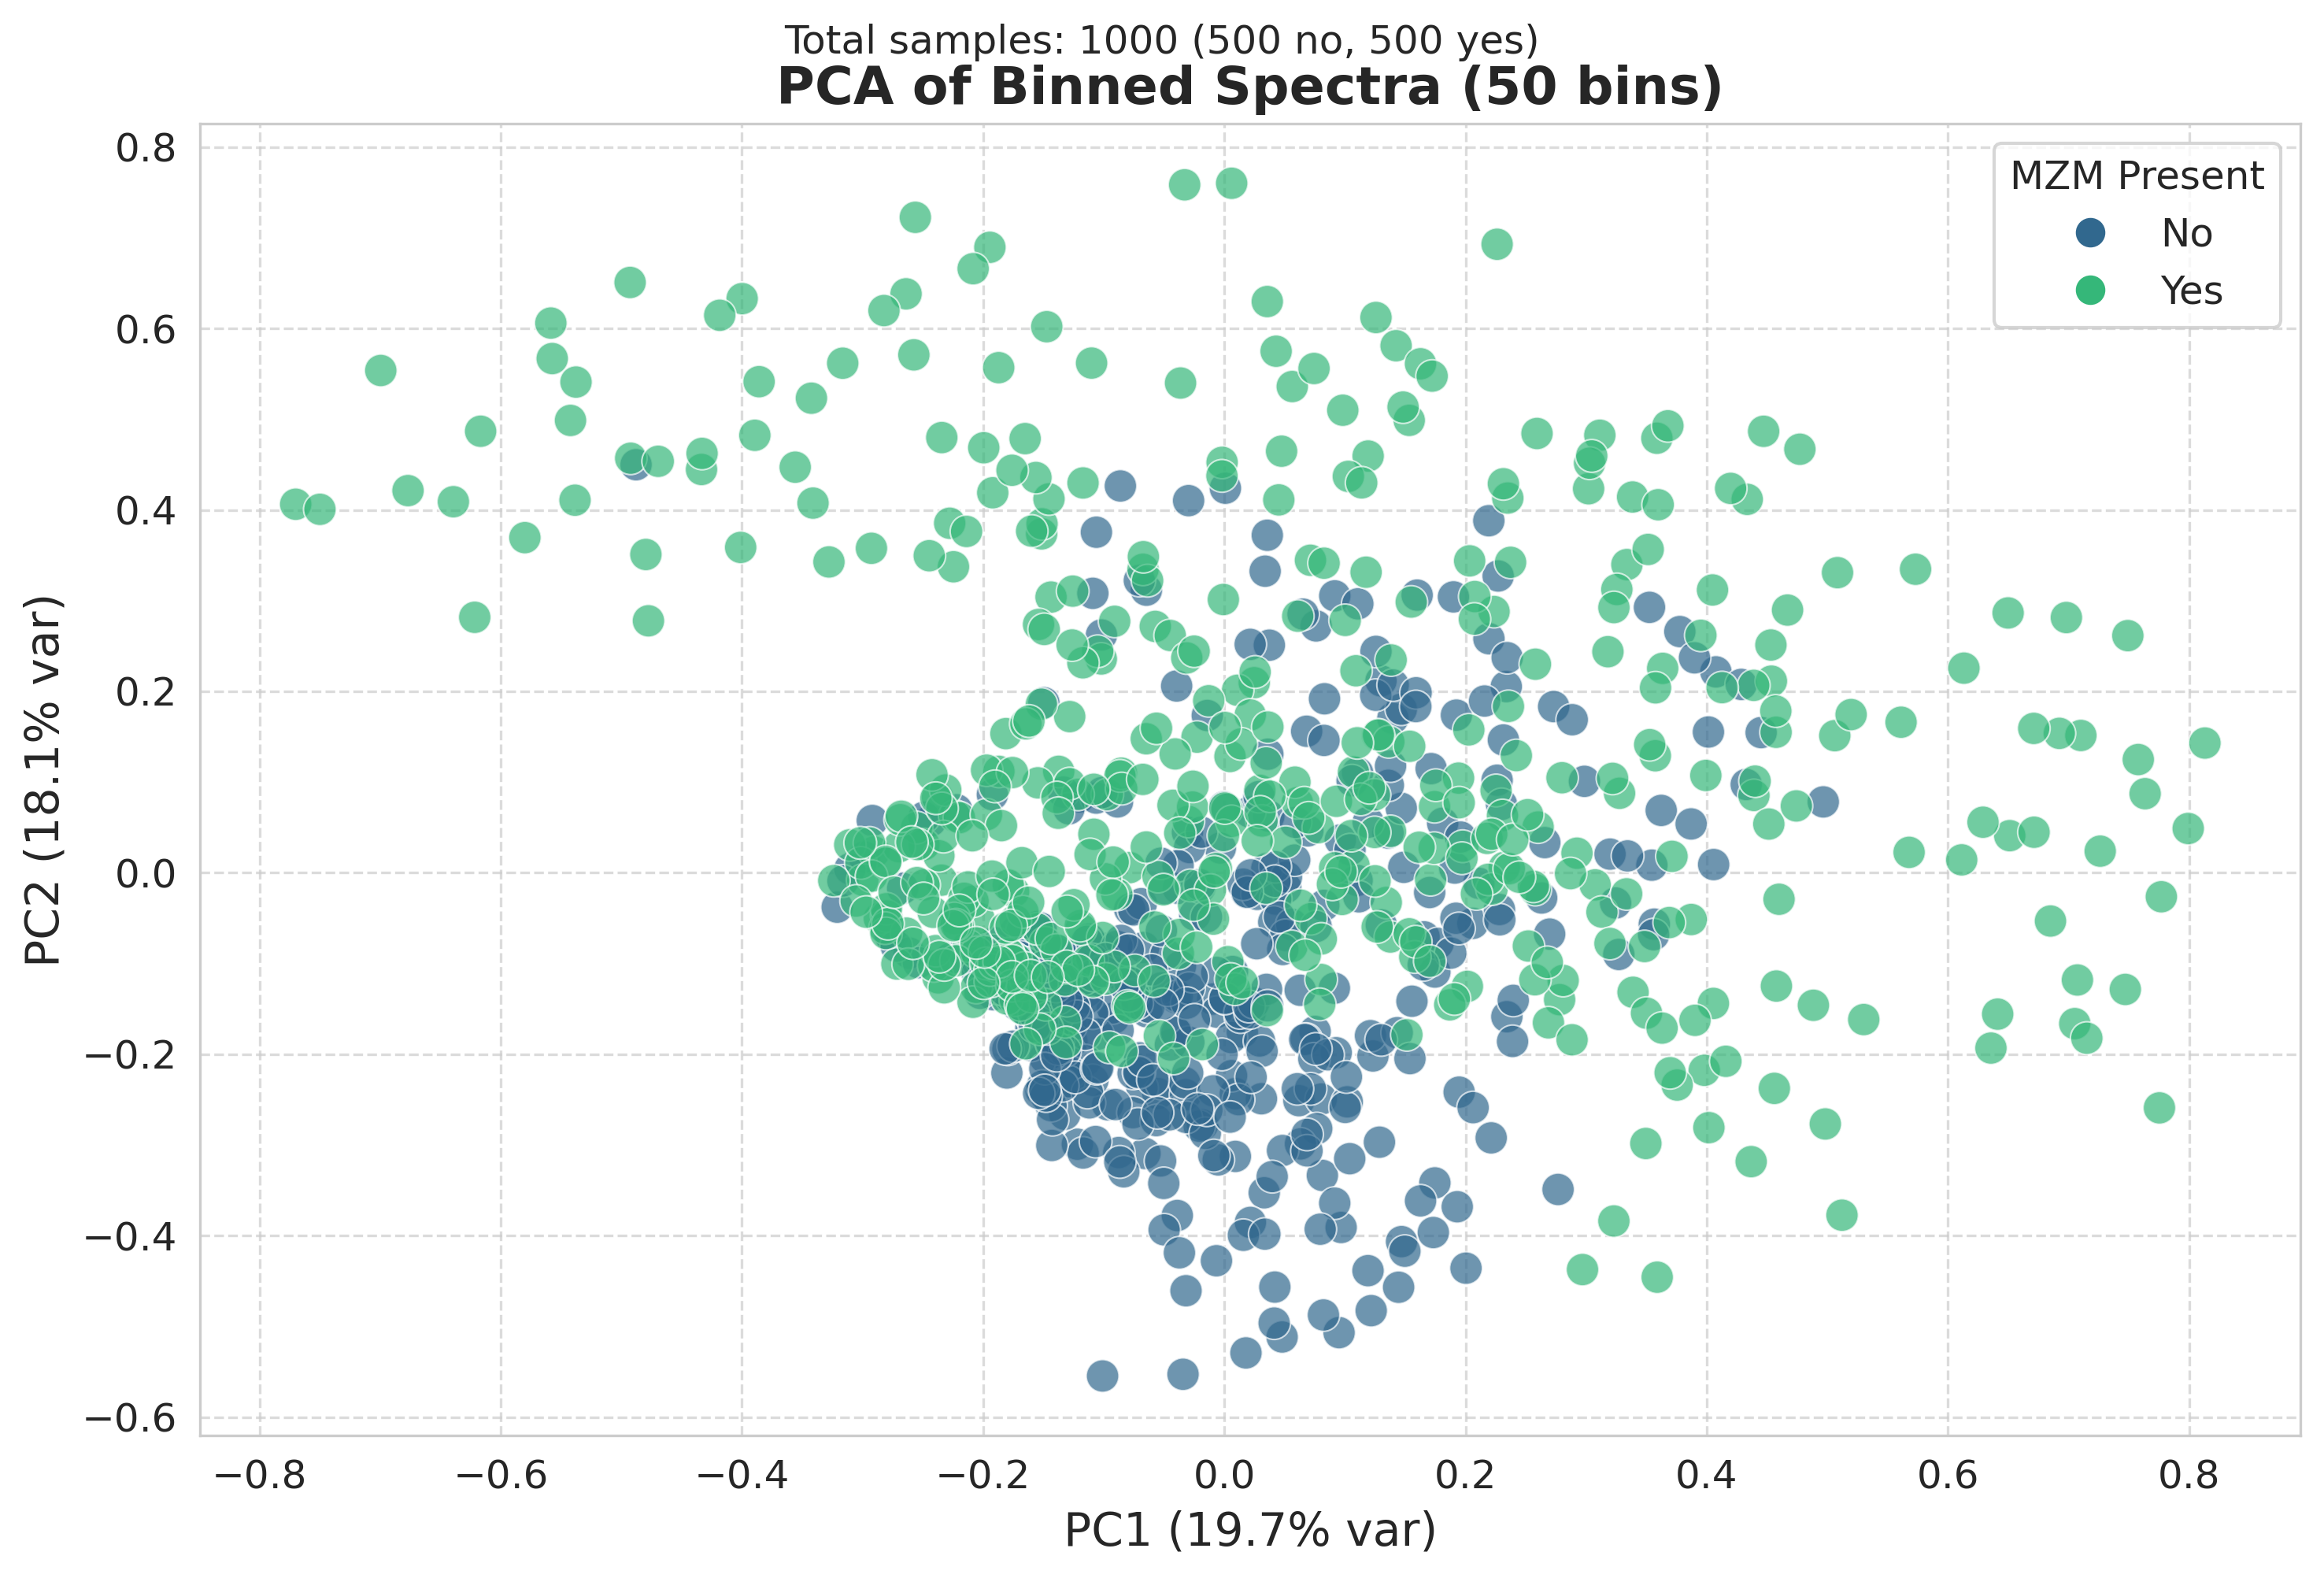
\includegraphics[width=0.65\textwidth]{pca_binned_spectra.png}
    \captionsetup{labelformat=empty,font=tiny}
    \caption{PCA of raw binned spectra (50 bins). PC1 and PC2 capture 19.7\% and 18.1\% of variance.}
  \end{figure}

  Using raw spectra results in poorer class separation compared to engineered features, highlighting the importance of feature engineering for MZM detection.
\end{frame}

\begin{frame}{PCA of Engineered Spectral Features}
  \tiny

  \begin{figure}
    \centering
    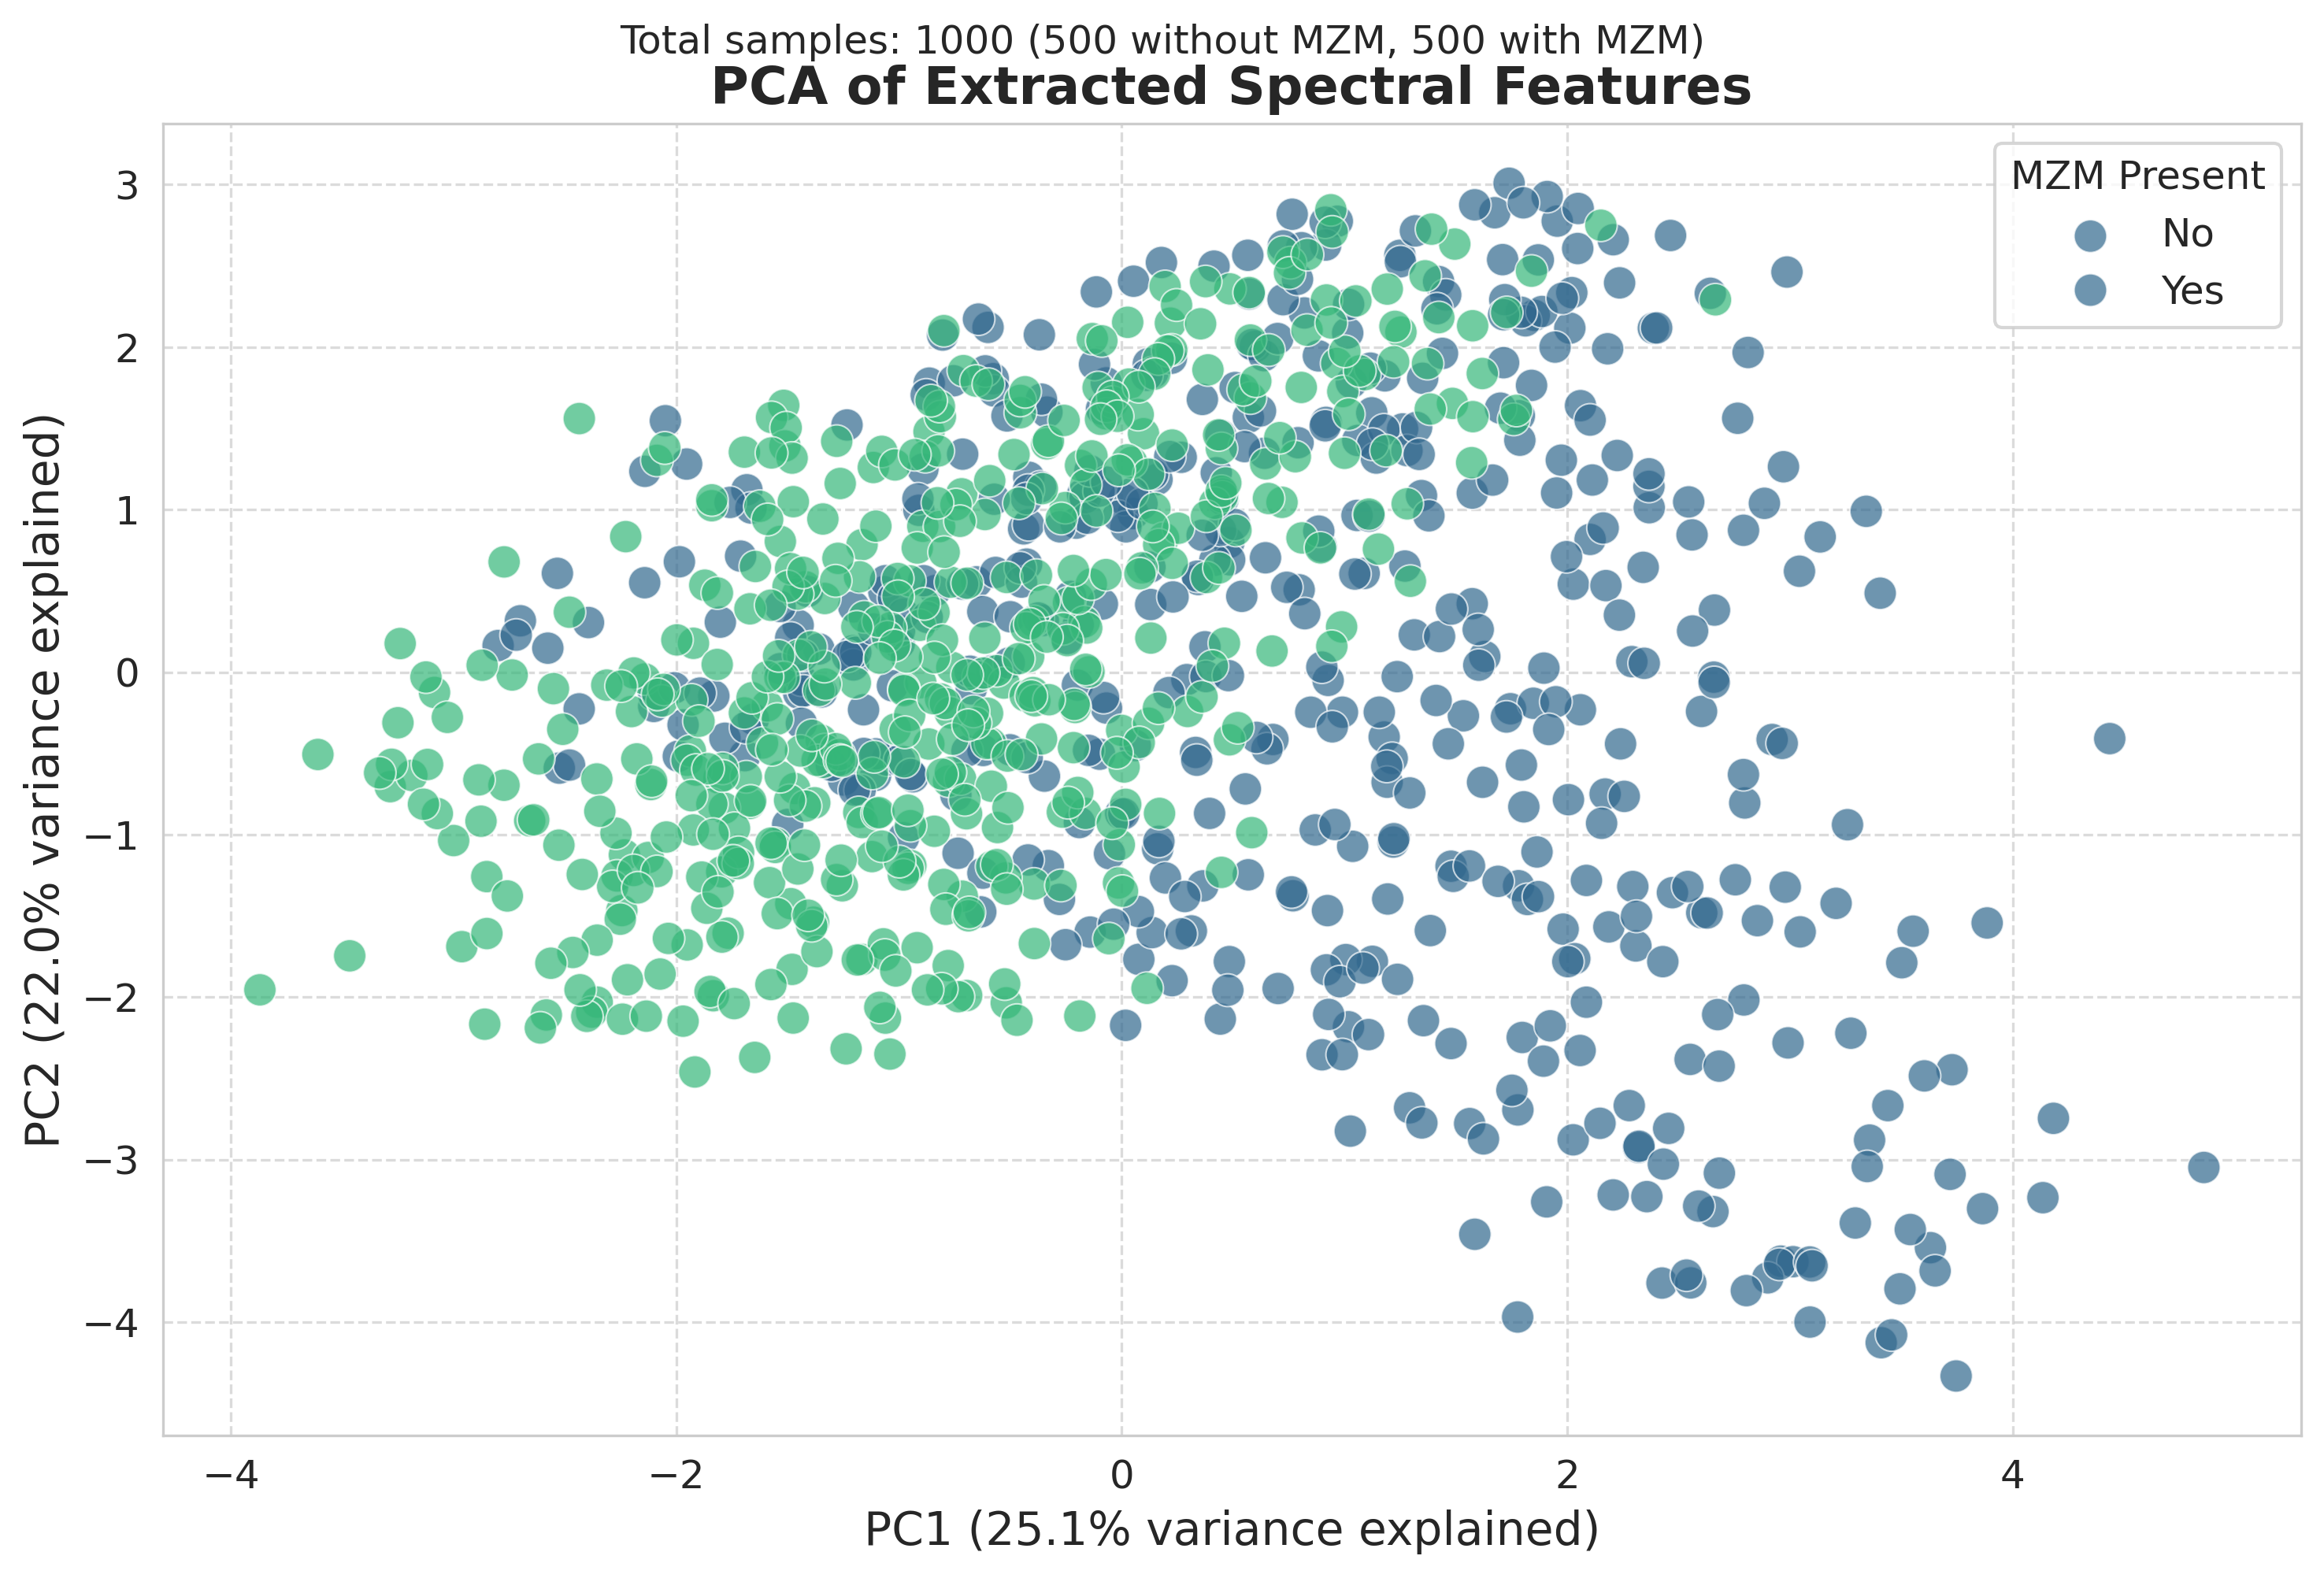
\includegraphics[width=0.65\textwidth]{pca_spectral_features.png}
    \captionsetup{labelformat=empty,font=tiny}
    \caption{PCA of engineered spectral features. Axes are the first two principal components (PC1, PC2), capturing 25.7\% and 21.5\% of variance.}
  \end{figure}

  The clear separation in this PCA plot shows that engineered features effectively distinguish MZM-hosting parameter sets, with PC1 and PC2 as arbitrary projections.
\end{frame}


\begin{frame}{Energy Spectrum with MZM}
  \tiny

  \begin{figure}
    \centering
    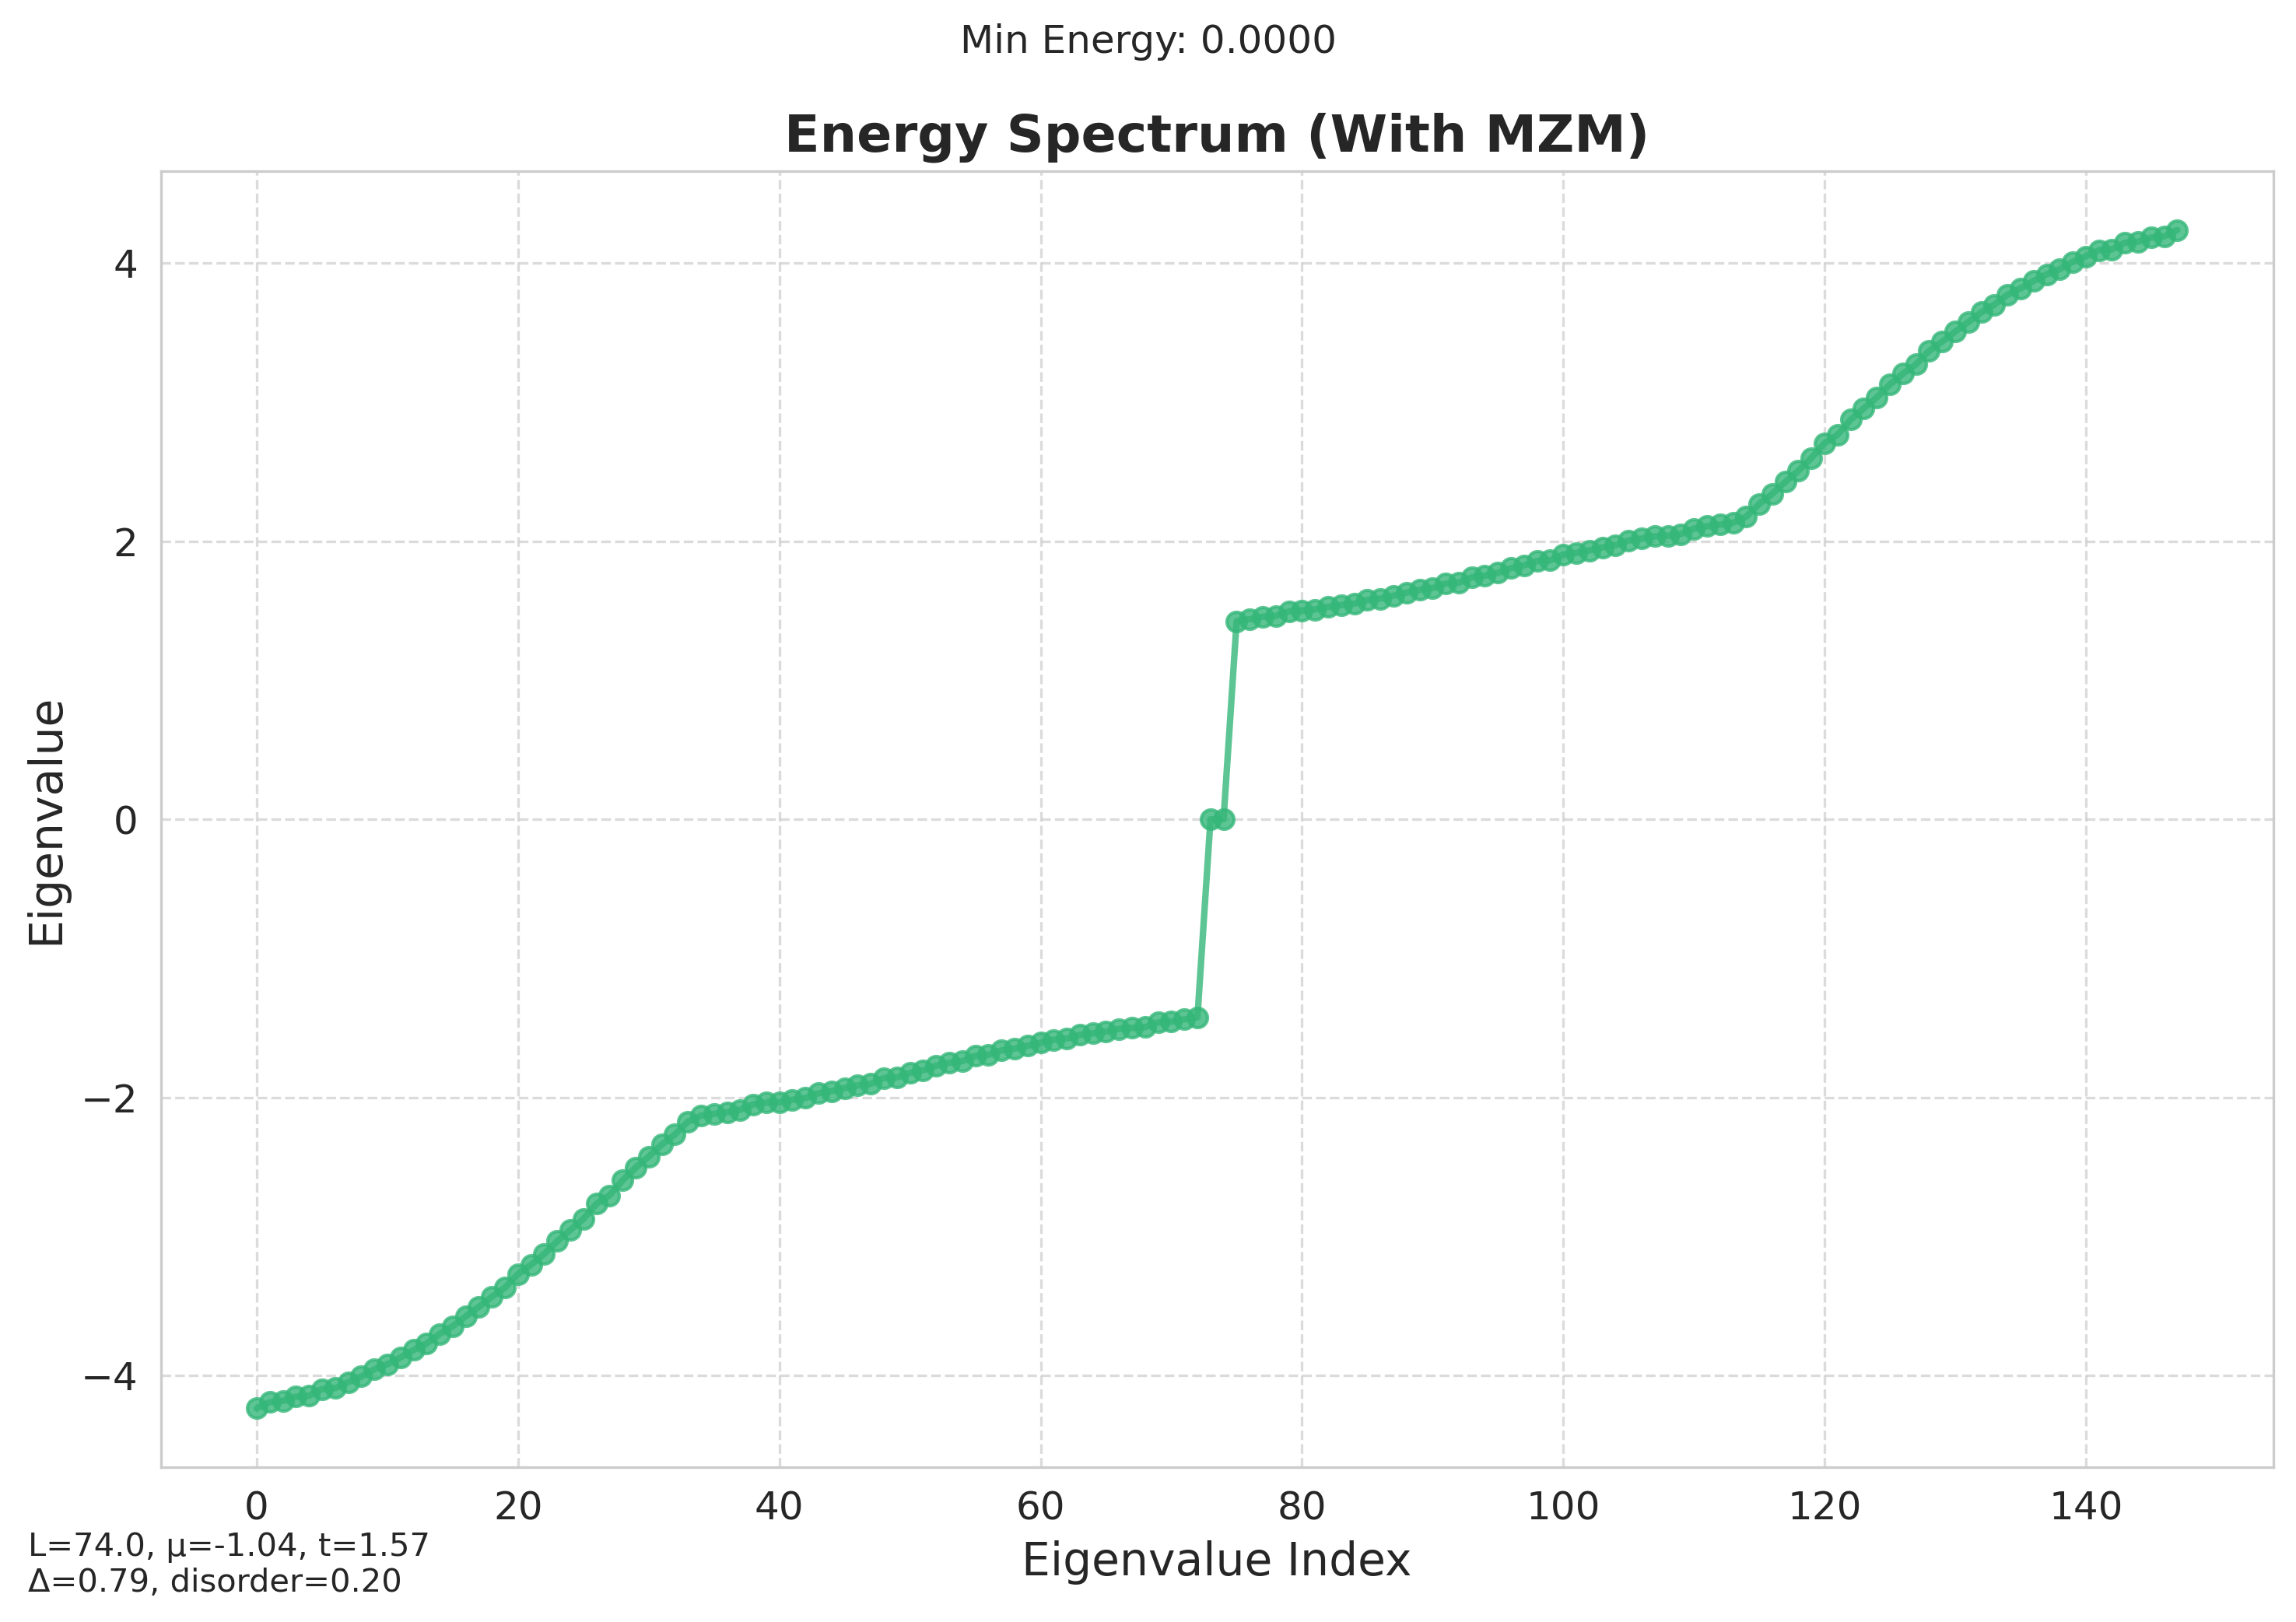
\includegraphics[width=0.65\textwidth]{spectrum_With MZM_train_3913.png}
    \captionsetup{labelformat=empty,font=tiny}
    \caption{Energy spectrum with an MZM. The $x$-axis indexes sorted eigenvalues; the $y$-axis gives eigenvalues in energy units (e.g., meV).}
  \end{figure}

  The spectrum shows a pair of states at or near zero energy, a hallmark of MZMs, distinguishing them from bulk states with finite energy gaps.
\end{frame}


\begin{frame}{Phase Diagram in $(\mu, \Delta)$ Plane}
  \tiny

  \begin{figure}
    \centering
    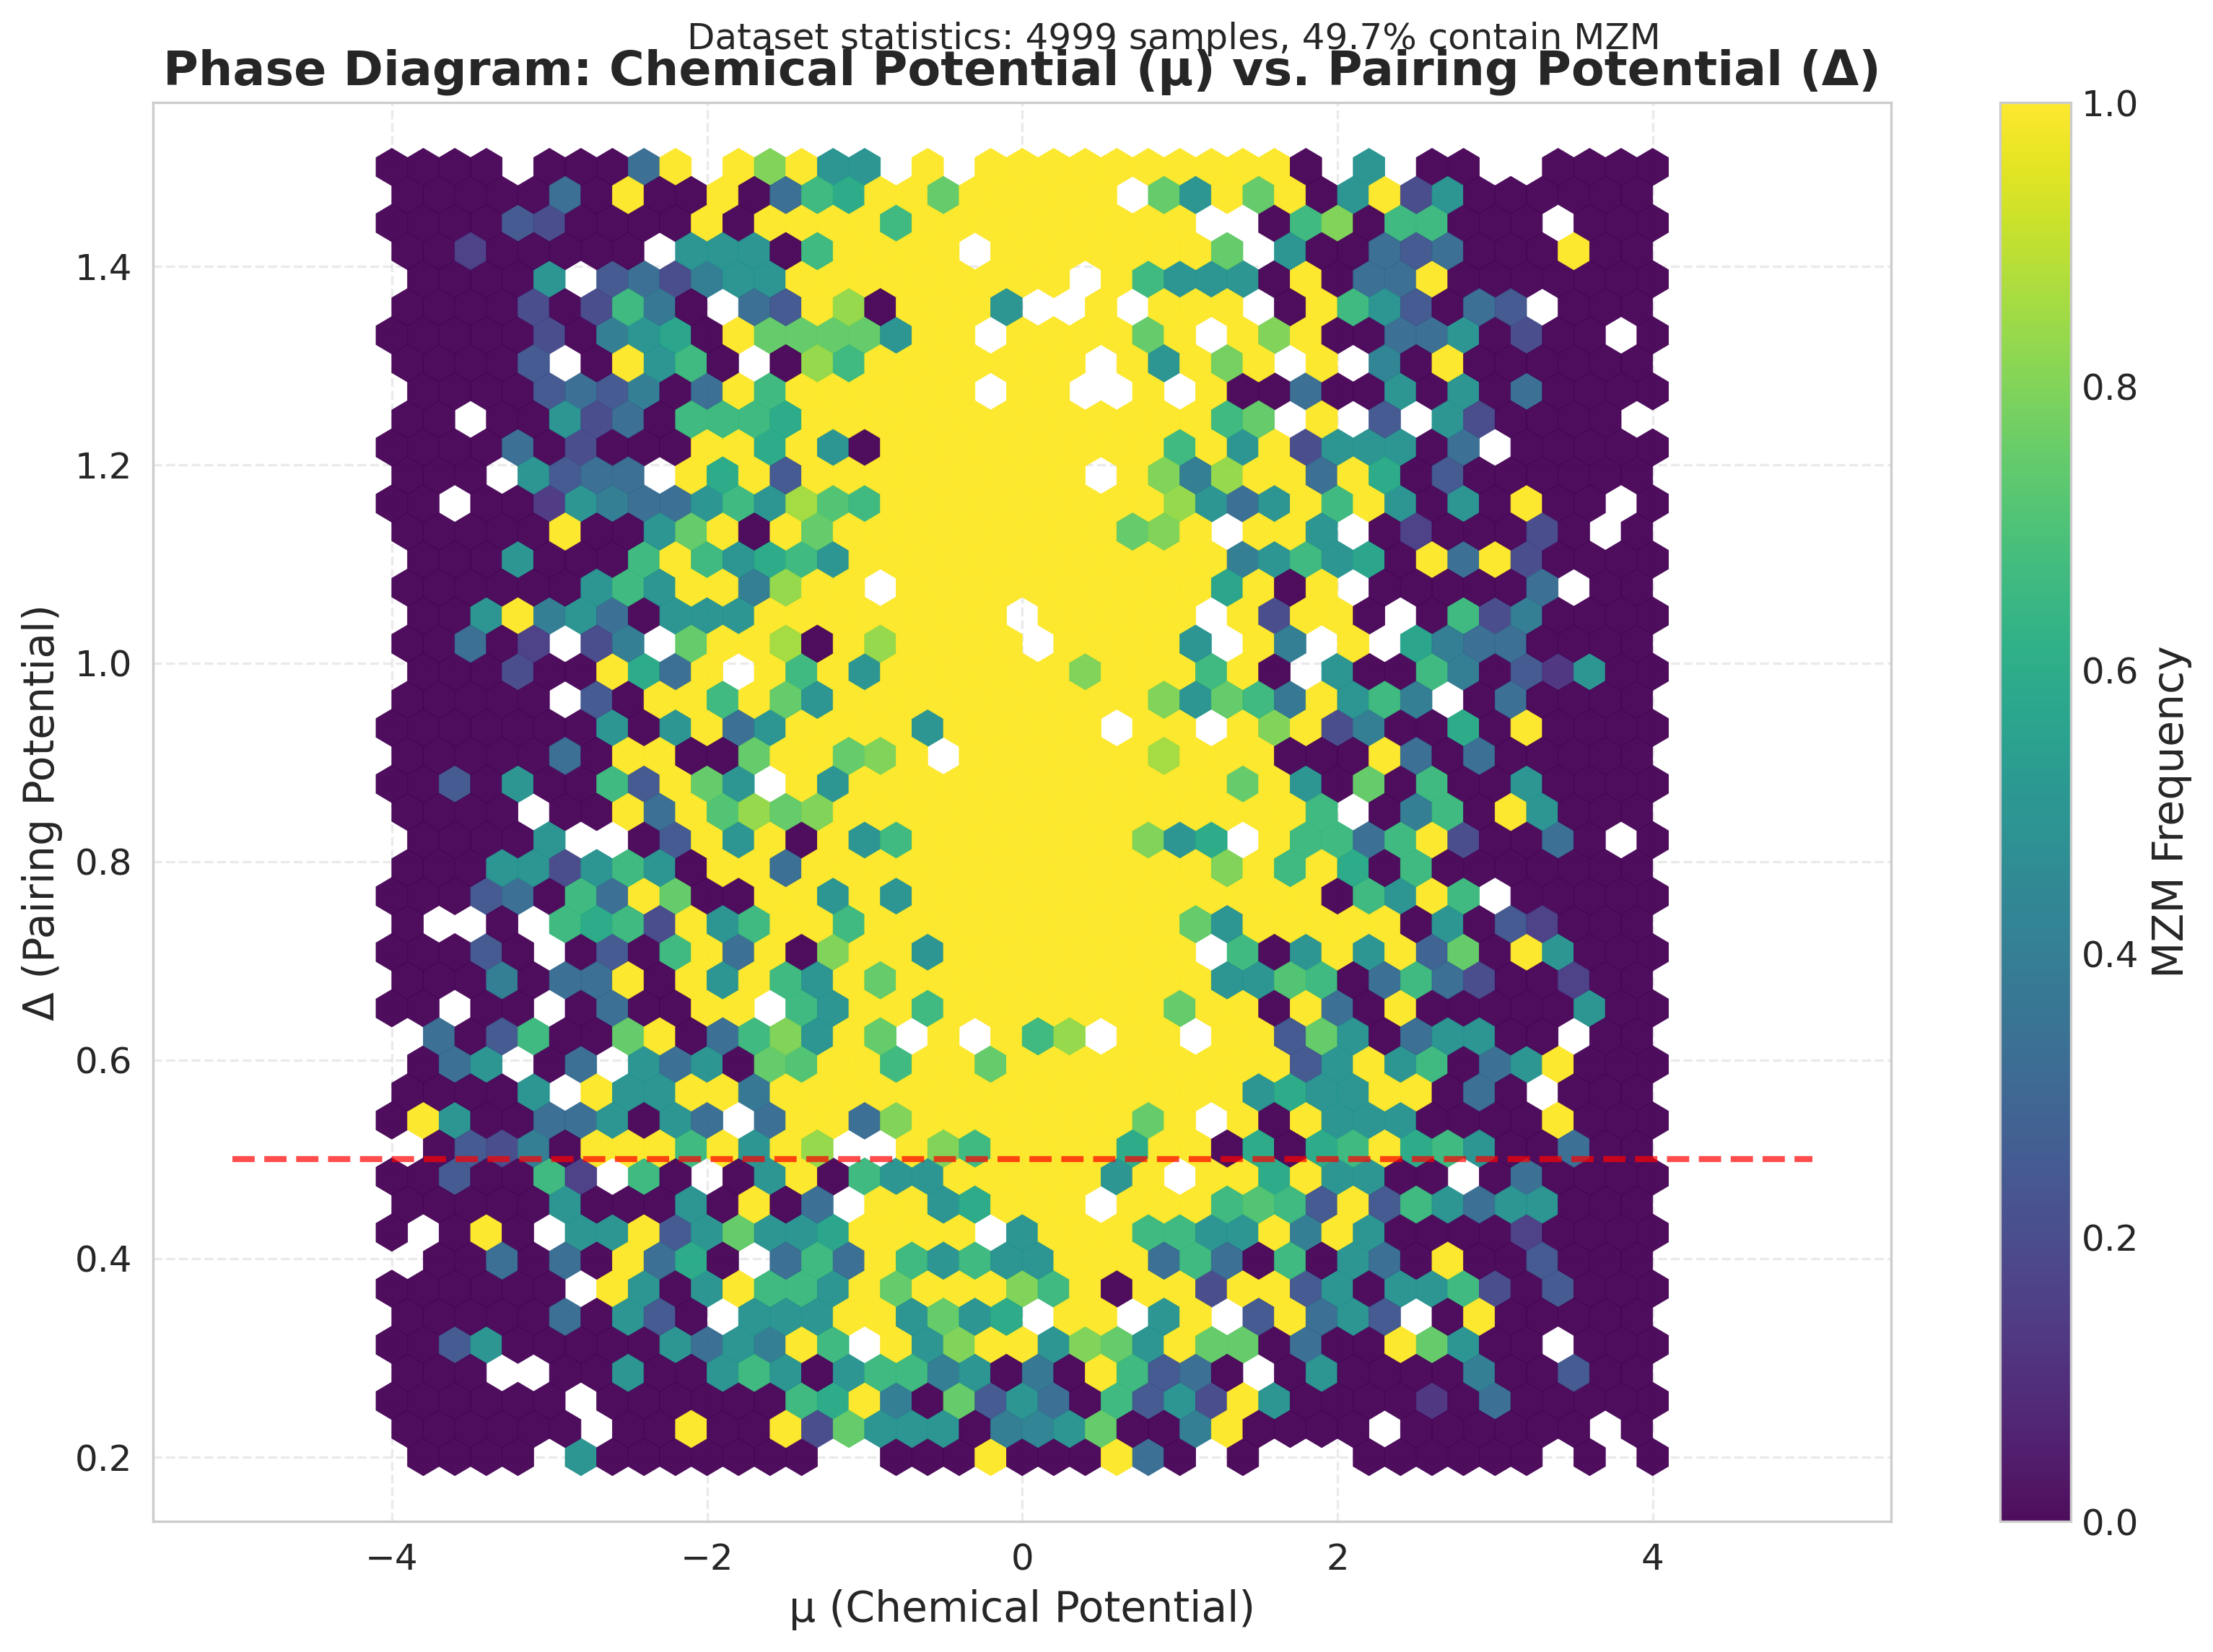
\includegraphics[width=0.65\textwidth]{phase_diagram_mu_delta.png}
    \captionsetup{labelformat=empty,font=tiny}
    \caption{Phase diagram in the $(\mu, \Delta)$ plane. The $x$-axis is $\mu$ (eV), the $y$-axis is $\Delta$ (eV), and color encodes MZM occurrence frequency.}
  \end{figure}

  This hexbin plot maps MZM occurrence, with the red dashed line at $\Delta = 0.5$ highlighting a region of high MZM probability, guiding parameter selection.
\end{frame}


% Summarizing diagnostics
\begin{frame}{Summary of MZM Diagnostics}
The diagnostics confirm MZM presence through:
\begin{itemize}
\item Bimodal edge-localization (histogram).
\item Clear separation in PCA with engineered features vs. raw spectra.
\item Zero-energy modes in the spectrum.
\item High MZM occurrence in specific $(\mu, \Delta)$ regions.
\end{itemize}
These results validate the Kitaev chain as a platform for studying topological superconductivity.
\end{frame}


\usepackage{booktabs}

\begin{table}[]
  \centering
  \caption{Architectural breakdown of \texttt{BdGPredictor}}
  \label{tab:enhanced-architecture}
  \begin{tabular}{@{}lccc@{}}
    \toprule
    \textbf{Stage}          & \textbf{Layer Type}   & \textbf{In\(\to\)Out} & \textbf{Remarks}                  \\
    \midrule
    Input                   & –                     & 5\(\to\)256           & Linear + GELU + Dropout          \\
    \emph{FeatureExtractor} & Linear                & 256\(\to\)512         & Residual proj., LayerNorm, Dropout \\
    \midrule
    Edge‐Loc Head           & Linear                & 512\(\to\)128         & GELU, LayerNorm                  \\
                            & Linear                & 128\(\to\)1           & Scalar output                    \\
    \midrule
    Spectrum Head           & Linear                & 512\(\to\)512         & GELU, LayerNorm                  \\
    (conv variant)          & Conv1D                & 16 ch × 32 len        & Residual conv block              \\
                            & Linear                & 512\(\to\)180         & Eigenvalue outputs               \\
    \bottomrule
  \end{tabular}
\end{table}



% Ending the document
\end{document}